\Introduction

Depuis l'apparition de l'informatique, les univers virtuels n'ont cessé de gagner en popularité, jusqu'à faire aujourd'hui partie intégrante de la société. Le domaine du divertissement a notamment beaucoup été impacté, conséquence de la grande liberté d'expression créative qu'offrent ces univers. Un des défis qui se dresse encore de nos jours est celui du remplissage de ces environnements. Ces derniers étant en constante expansion, les méthodes de création de contenu traditionnelles, par le travail manuel des artistes, atteignent leurs limites, et appellent à la mise au point de nouveaux moyens plus automatisés pour permettre une création plus rapide et moins coûteuse. 

\begin{figure}[!h]
    \centering
    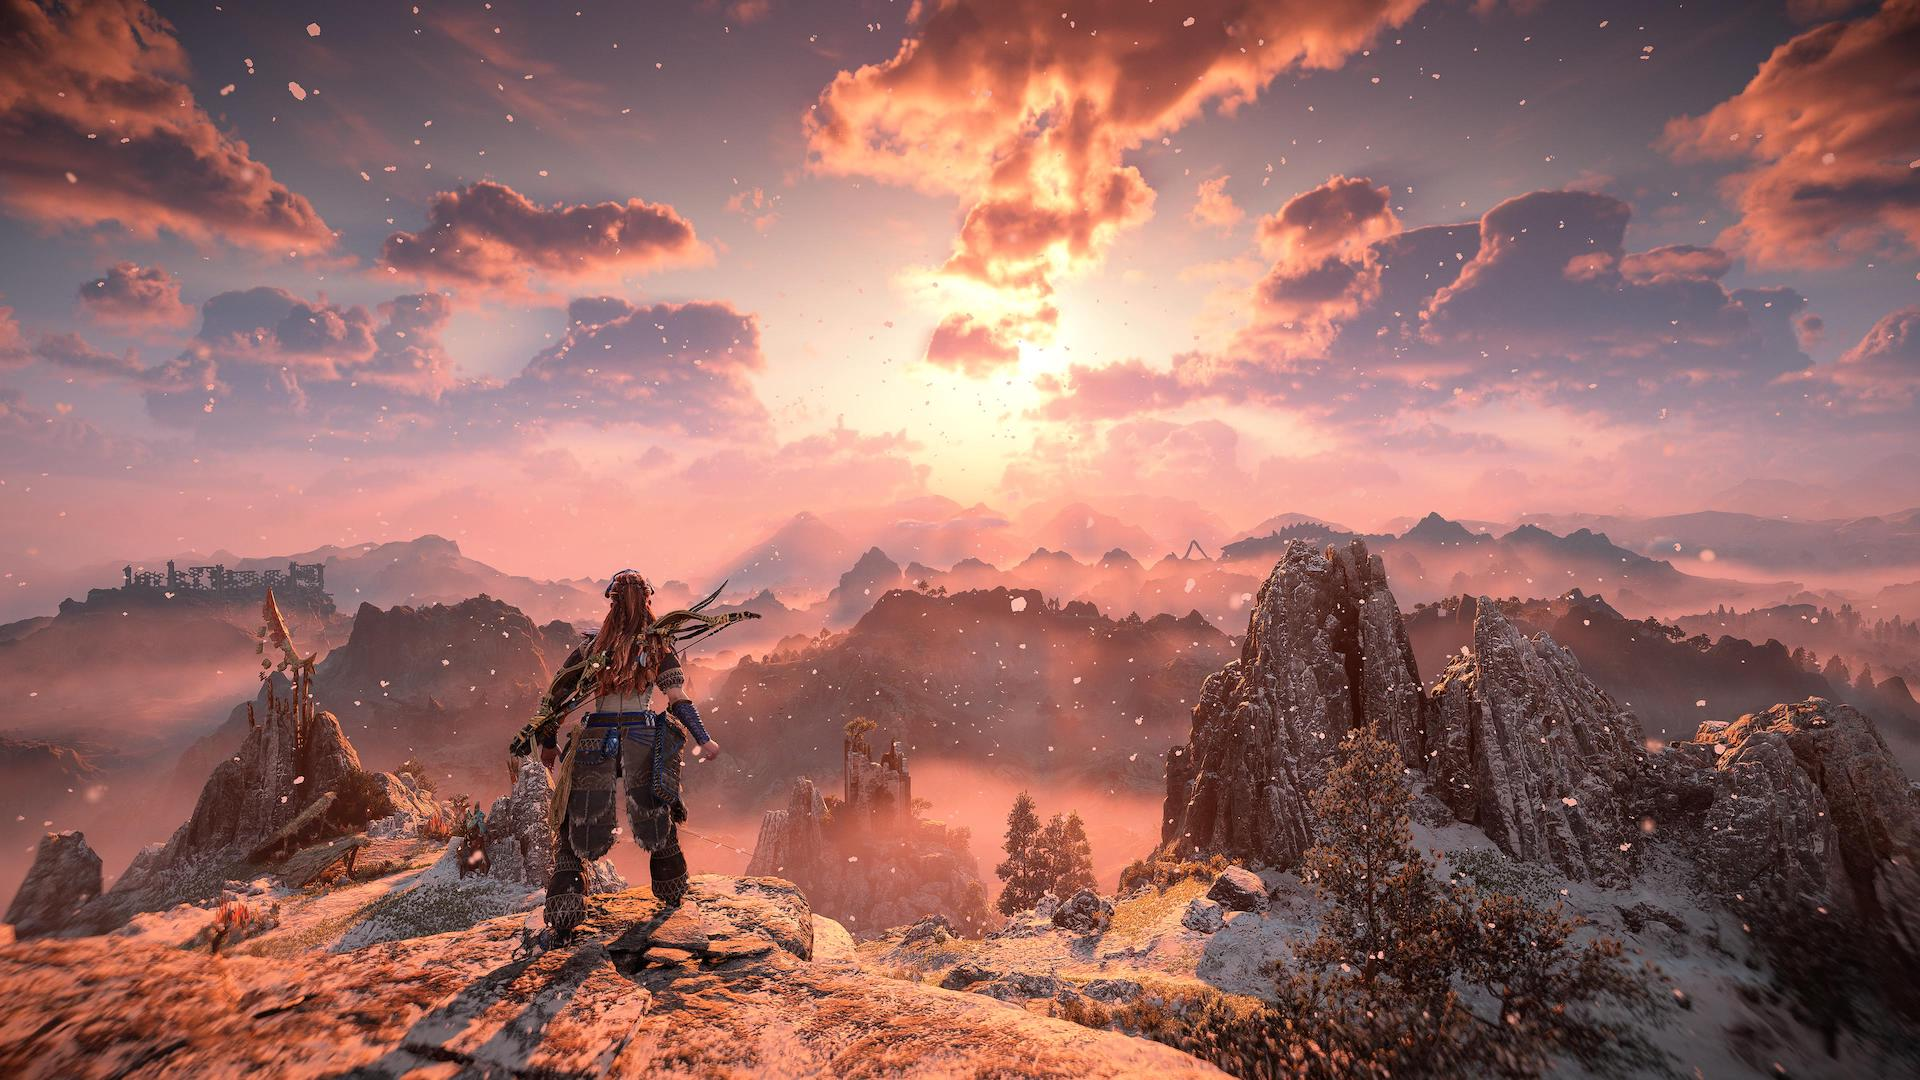
\includegraphics[width=.75\textwidth]{contenu/resources/images/Horizon-Forbidden-West}
    \caption{{\it Horizon Forbidden West} (2022), Guerilla Games}
    \label{fig:horizon}
\end{figure}

Dans ce contexte de méthodes automatisées, la génération procédurale est un procédé utilisé pour produire toutes sortes de ressources, et notamment pour synthétiser l'apparence visuelle des différents composants des scènes virtuelles. En combinant des méthodes algorithmiques avec de l'aléatoire, on génère des cartes de texture qui servent à habiller les mondes virtuels, en améliorant l'apparence visuelle et en accentuant l'immersion. Différentes textures nécessitent différentes méthodes de synthèse, et certains genres de textures sont encore difficilement réalisables avec les méthodes existantes. C'est dans cette perspective que s'inscrit ce travail de recherche, qui a pour but d'approfondir notre compréhension des éléments qui constituent la structure d'une image. On s'appuie pour cela sur l'étude exploratoire de l'analyse multi-résolutionnelle, outil du domaine du traitement du signal, et de son application à la synthèse de texture.

\section{Monde virtuel}

Un monde virtuel est une méthode de représentation de scènes, réelles ou imaginées, au moyen d'un support numérique. Ces scènes sont composées de collections d'objets numériques qui intéragissent entre eux, comme des surfaces, des personnages, des lumières, des caméras, et d'autres encore. Il existe de nombreux types de monde virtuel différents, qui varient en taille, en mode de représentation, ou encore en genre d'objets représentés. Ils sont en effet utilisés dans de nombreux domaines, comme par exemple :

\begin{itemize}
    \item le domaine du divertissement, pour les jeux vidéo (l'industrie du jeu-vidéo est un des principaux acteurs des avancées en graphisme) ;
    \item le domaine de l'animation, pour les films d'animation ou les effets spéciaux de films ;
    \item le domaine médical, pour des outils de visualisation de l'anatomie humaine ou de formation en réalité virtuelle ;
    \item le domaine de l'ingénierie, pour aider à la conception d'objets (Conception Assistée par Ordinateur) ou de bâtiments (architecture) ;
    \item le domaine militaire, pour faire des simulations de situations ou des entraînements au combat.
\end{itemize}

\subsection*{Types de rendu}

Pour visualiser les scènes virtuelles, on utilise un moteur de rendu, un logiciel utilisant différents algorithmes permettant de traiter une scène en différentes étapes dans le but de synthétiser une image ; ce que l'on appelle le rendu de la scène. Il existe plusieurs méthodes de rendu, et plusieurs moteurs différents qui implémentent ces méthodes en fonction du niveau de réalisme attendu, des effets visuels présents dans la scène, mais surtout en fonction du type d'application désiré. Pour exécuter leurs calculs, les logiciels de rendu s'appuient sur les capacités des cartes graphiques ({\it Graphics Processing Unit} ou GPU en Anglais), des processeurs hautement parallèles et spécialisés pour des calculs graphiques. On distingue deux grands types de rendus, dont les contextes et enjeux diffèrent sensiblement :

\begin{figure}[h!]
    \centering
    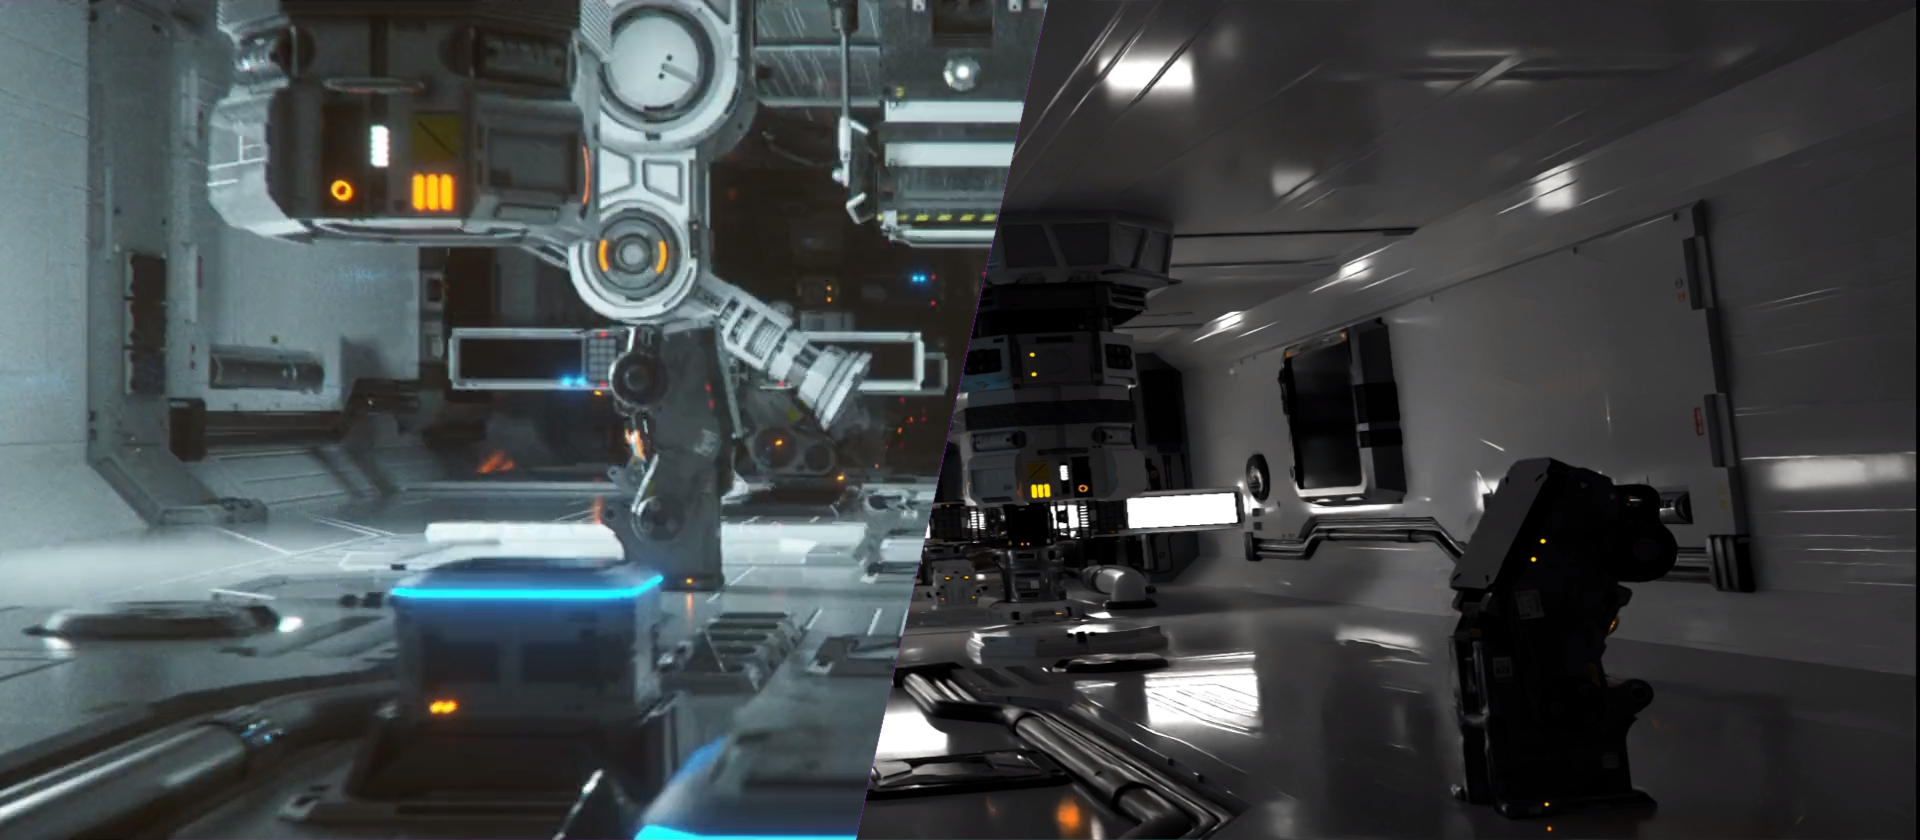
\includegraphics[width=\textwidth]{contenu/resources/images/zero_day_comparison}
    \caption[{\it Zero-Day} (2015), BEEPLE]{{\it Zero-Day} (2015), BEEPLE. À gauche rendu original hors-ligne, à droite rendu temps-réel par SY tracé de chemins, NVIDIA~\cite{ZeroDay}}
    \label{fig:zero-day}
\end{figure}

\begin{itemize}
    \item le rendu hors-ligne (ou pré-calculé), utilisé pour représenter des scènes non-interactives, des images ou des films. Le rendu est souvent complexe et de très haute qualité, mais utilise des algorithmes gourmands en ressource et nécessitant un long temps de calcul. Toute éventuelle animation de la scène ou déroulement de l'action est pré-déterminé, tout est calculé lors du rendu.
    \item le rendu intéractif (ou temps-réel), utilisé pour traiter des scènes interactives, comme des jeux vidéo ou des simulations. Le rendu privilégie la performance car la scène évolue en fonction des entrées de l'utilisateur, qui manipule l'application en même temps que le rendu se fait. Le rendu doit donc être assez performant pour pouvoir afficher les images de telle sorte que le flux soit continu à l'oeil humain. Le minimum est à 24 images par secondes, mais en pratique les applications visent des objectifs d'au moins 30 ou 60 images par secondes, soit un budget temps de 33,3 à 16,6 ms par image. La qualité des graphismes est donc délaissée au profit de l'efficacité pour atteindre le taux de rafraîchissement cible. Les algorithmes utilisés doivent ainsi être conçus pour s'exécuter avec moins de temps, moins de ressources de calcul, et moins d'espace mémoire disponible.
\end{itemize}

\bigskip

% Blurring the line between real-time / offline
Ces deux types de rendus sont ainsi très différents, et les méthodes dévelopées pour l'un ne s'appliquent pas, ou pas directement, à l'autre. Les avancées dans le domaine de l'informatique graphique et dans celui des GPUs rapprochent cependant de plus en plus ces méthodes. Le travail exposé dans ce manuscrit vise à explorer un outil pour le rendu temps-réel, les solutions et problématiques concernant le rendu hors-ligne serons donc mises de côté.

{\color{red}est ce qu'on positionne tel quel ? Construction de pyramide et PC sont plutot offline...}

\subsection*{Maillage}

Idéalement, on aimerait représenter les objets des scènes (d'un monde ) virtuel(les) de manière continue et exacte, mais une telle représentation est difficilement accessible. Comme solution pratique, on choisit d'utiliser des maillages, des grilles de polygones (souvent des triangles) qui sont une approximation de notre géometrie, approximation dont la complexité et la densité peuvent varier selon les besoins. Les maillages étant SY stockés comme des tableaux de points et de faces, il se pose en effet des questions de coût en espace mémoire et de tractabilité des calculs qui sont effectués sur ces maillages par la suite, surtout dans le cas du rendu temps réel.

\begin{figure}[h!]
    \centering
    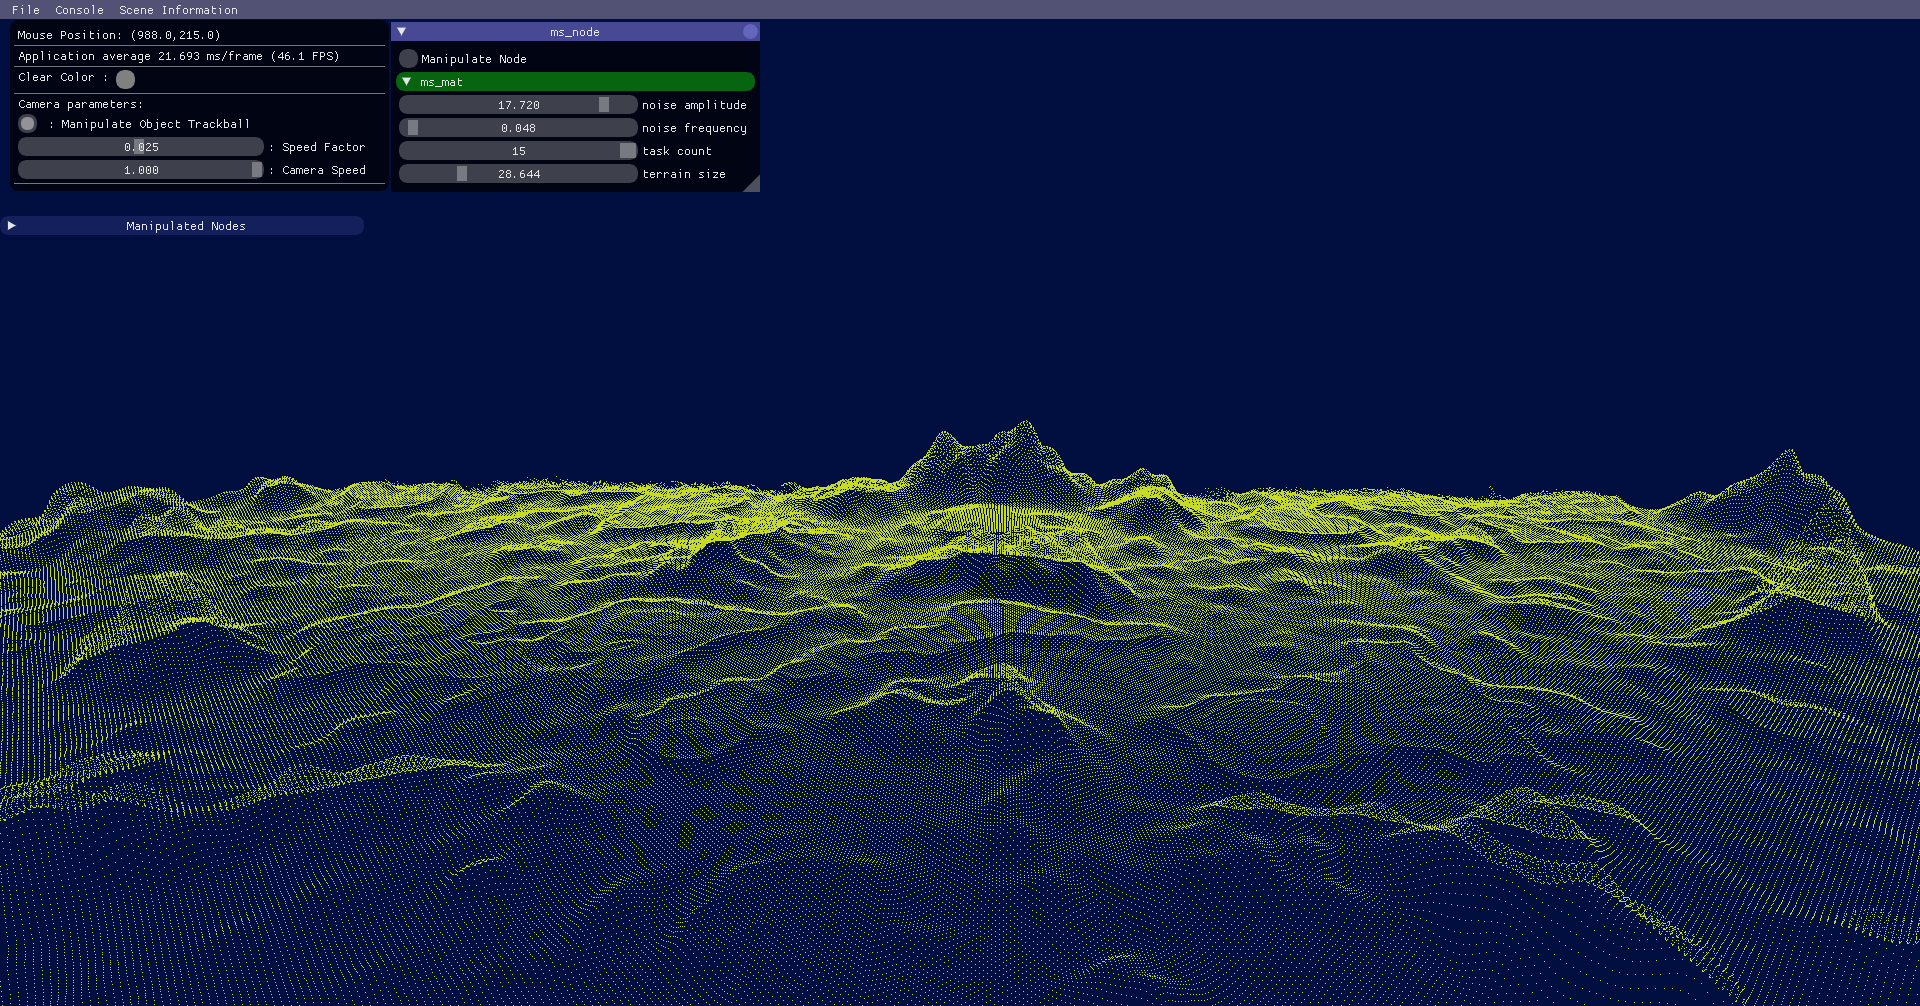
\includegraphics[width=\textwidth]{contenu/resources/images/full_terrain}
    \caption{Maillage d'un terrain généré procéduralement}
    \label{fig:procedural-mesh}
\end{figure}

\section{Texture}

\subsection*{Plaquage de texture}

Le maillage seul ne suffit cependant pas à représenter parfaitement la géometrie (micro mesh goes hehe), qui a trop de détails pour la résolution des maillages tractables avec la technologie actuelle. Pour remédier à ce problème, on utilise des textures, qui ajoutent les détails manquants à une géometrie simplifiée. De manière générale, on appelle texture une fonction d'un espace de coordonnées, souvent deux ou trois dimensions, vers un espace de valeurs numériques à une ou plusieurs dimensions. Les dimensions de l'espace d'arrivée sont appelées canaux de la texture. Ils représentent souvent une couleur (RGB ou RGBA), mais peuvent aussi correspondre à d'autres grandeurs (scalaires par exemple) qui encodent des valeurs physiques utiles au rendu de la scène, comme une profondeur, une hauteur, ou un vecteur normal par exemple. La majorité du temps, les textures sont stockées en mémoire comme des images, des tableaux finis de données multi-dimensionnels, que l'on appelle alors des cartes. 

\bigskip

Pour une même surface, il est courant d'utiliser plusieurs textures pour calculer l'éclairage et la couleur. Les textures en question dépendent du modèle d'éclairage utilisé. Le format de rendu physique réaliste ({\it Physically Based Rendering} ou PBR en Anglais), standard de l'industrie, nécessite typiquement cinq cartes de texture : l'albedo (ou couleur), mais aussi la normale, la hauteur, la rugosité et l'occlusion ambiante. 

\begin{figure}
    \centering
    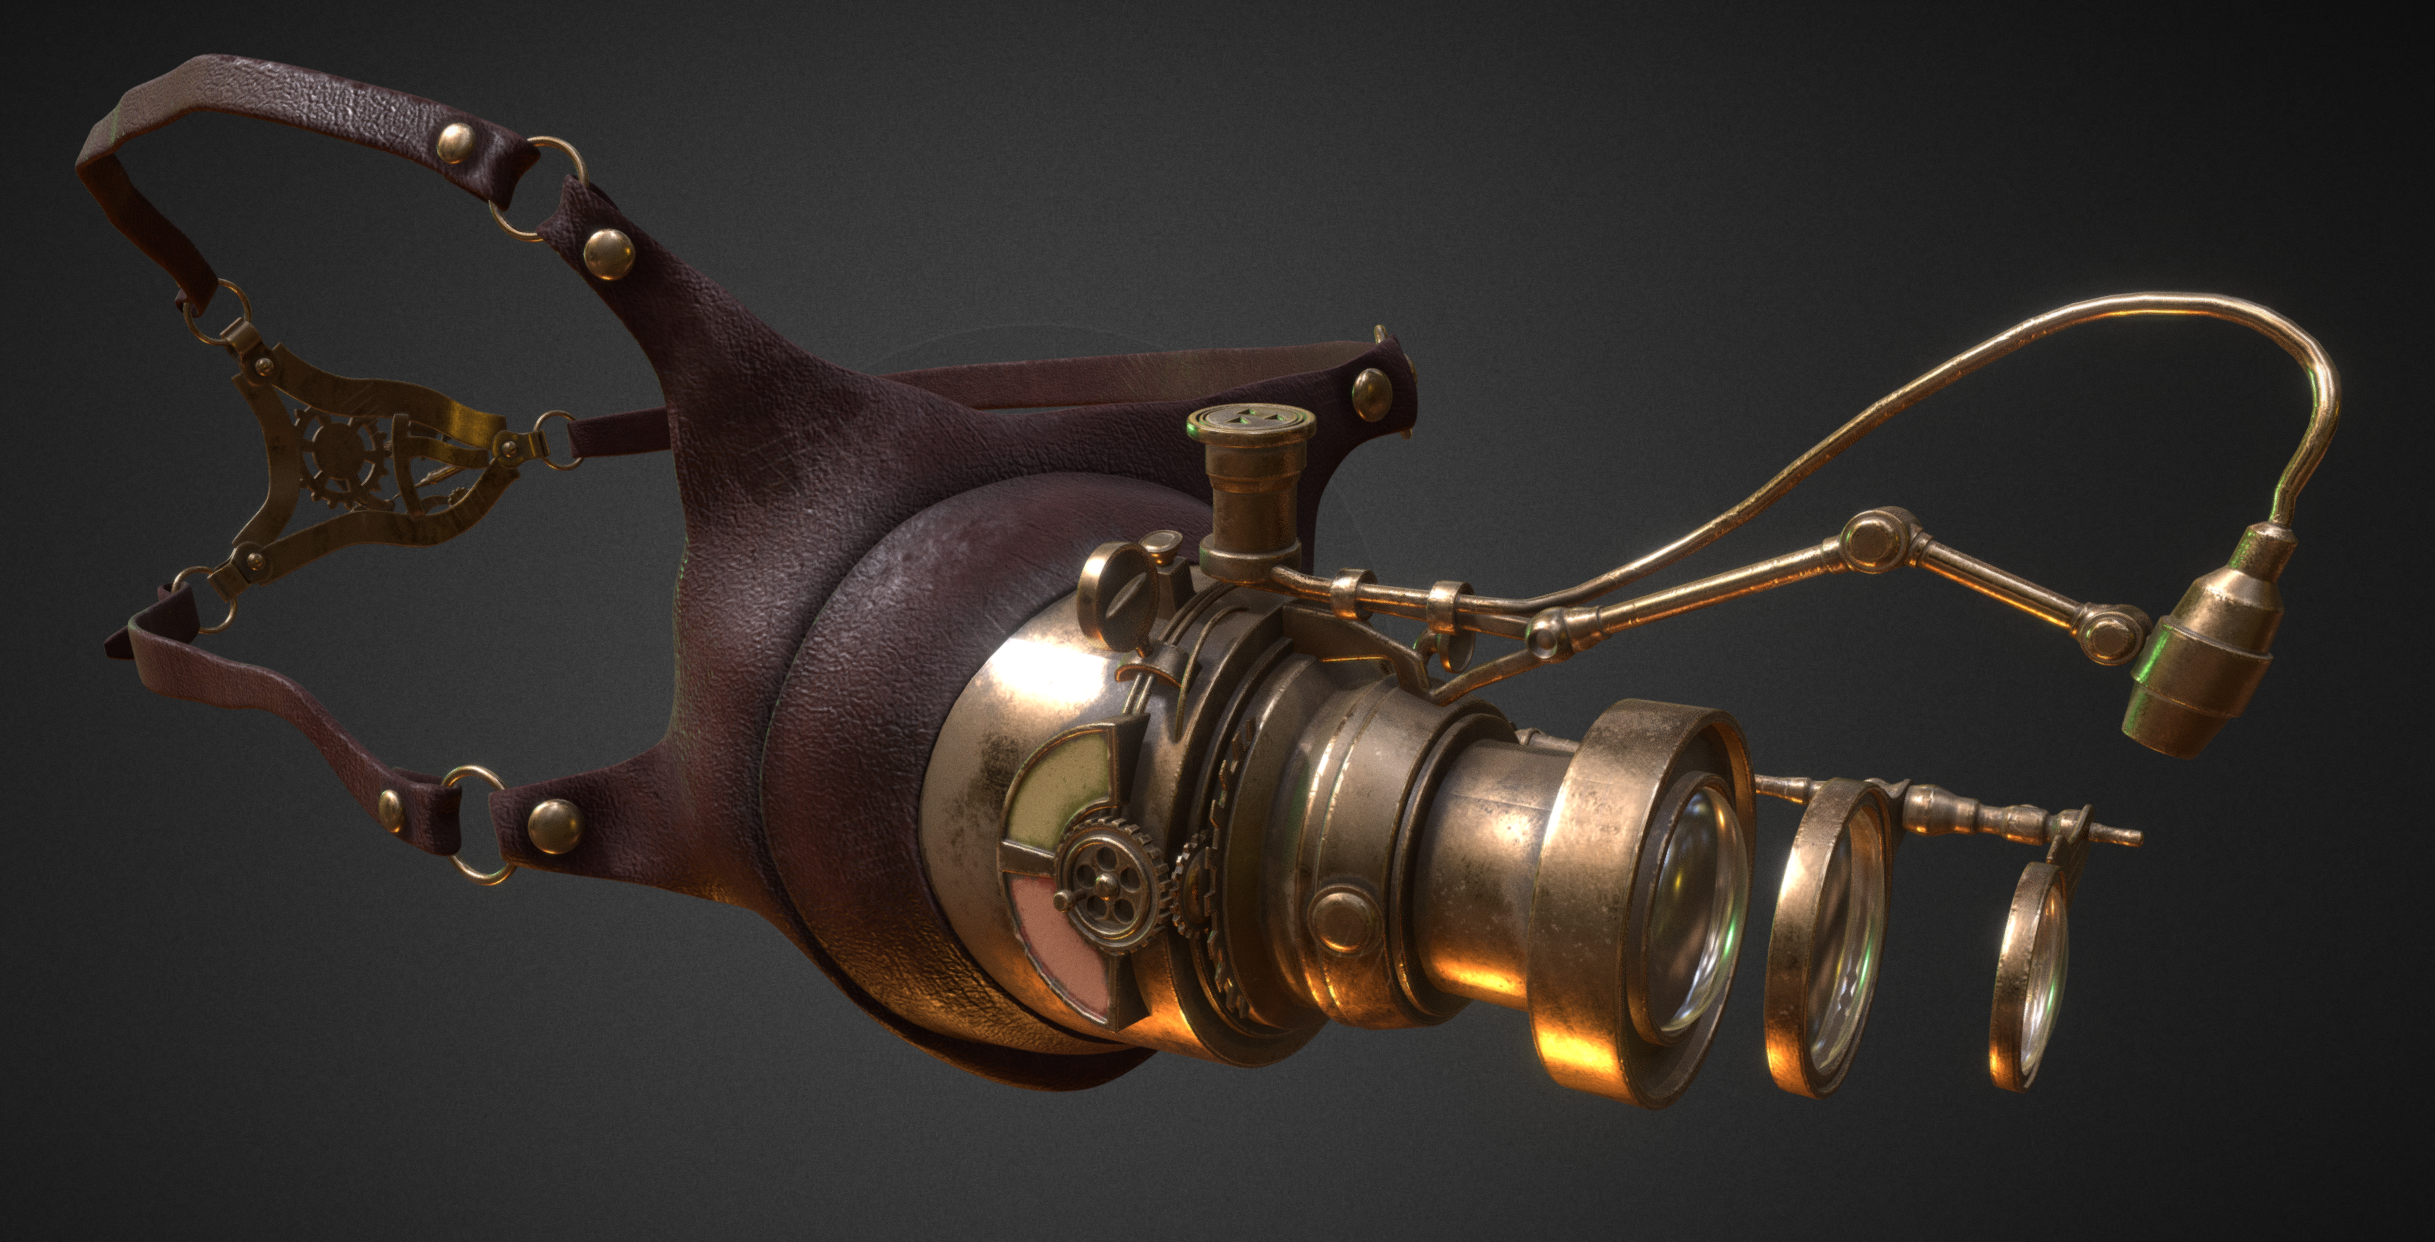
\includegraphics[width=.65\textwidth]{contenu/resources/images/mutli-material-object}
    \caption[Rendu d'un objet comportant plusieurs matériaux]{Plusieurs matériaux différents sont utilisés pour le rendu de cet objet~\cite{multi-material}}
    \label{fig:multi-material}
\end{figure}

La méthode de travail usuelle en industrie consiste à regrouper ces différentes textures, ainsi que le modèle d'éclairage, dans un matériau. Les objets d'une scène sont ainsi composés de plusieurs matériaux, qui présentent chacun des propriétés physiques différentes. Une chaise peut par exemple avoir une armature en bois, un recouvrement en cuir et des clous en métal. Pour créer leurs scènes, les artistes façonnent ainsi leurs objets en commençant par la géométrie, avant de créer (ou réutiliser) les différents matériaux pour habiller leurs objets.

\subsection*{Échantillonnage}

L'intérêt de la texture est donc d'augmenter la quantité de détails de notre rendu à faible coût, puisque la géometrie sous-jacente reste plus grossière, et que la résolution de cette dernière est un des facteurs majeurs de ralentissement du rendu d'une scène. Pour plaquer des textures, qui souvent sont des images carrées, sur une surface quelconque, on utilise un système de coordonnées, dites UV, qui permet d'aligner les deux comme souhaité. Les coordonnées UV, un vecteur entre $(0, 0)$ et $(1, 1)$, sont définies pour tous les sommets au moment de la création du maillage. On peut alors utiliser ces coordonnées comme argument de la texture, dont l'espace de coordonnées de départ est aussi entre 0 et 1.

\begin{figure}
    \centering
    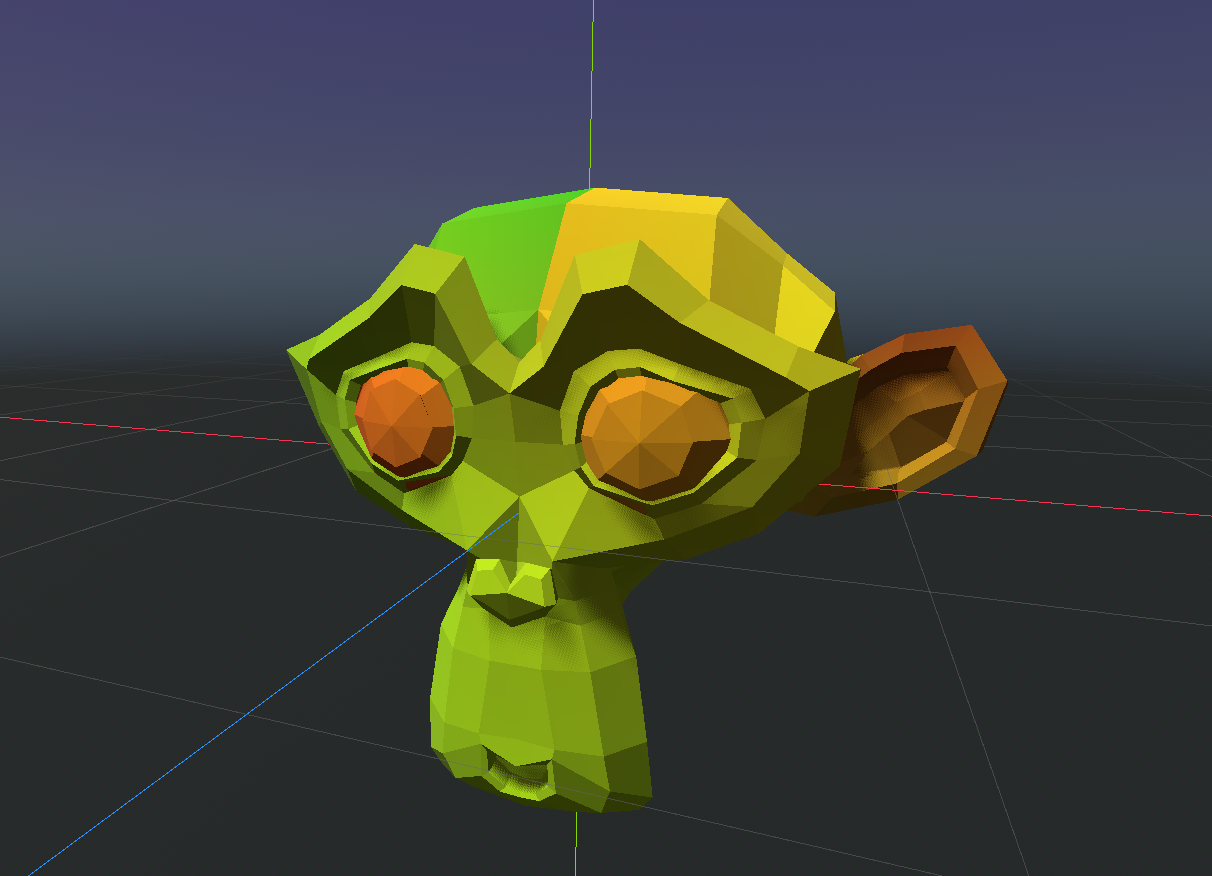
\includegraphics[width=.55\textwidth]{contenu/resources/images/uv_suzanne}
    \caption[Coordonnées UV du modèle Suzanne]{Visualisation des coordonnées UV de Suzanne~\cite{suzanne-uv}, modèle 3D de référence du logiciel Blender}
    \label{fig:uv-suzanne}
\end{figure}

Cette étape dite d'échantillonnage s'effectue au moment du rendu. Dans la pipeline graphique de rastérisation, utilisée classiquement pour faire du rendu intéractif, la scène est projetée sur le plan image, puis découpée en fragments de taille inférieure aux polygones formant le maillage des objets de la scène. Les fragments ont une valeur de coordonnée UV, interpolée entre les valeurs des sommets voisins, et peut donc aller interroger les textures pour récupérer les valeurs aux bons endroits. 

\subsection*{Filtrage}

Cette méthode pose cependant des problèmes dûs à l'encodage discret des textures en image. En effet les fragments rastérisés et les texels de texture échantillonnés représentent tous les deux des surfaces de petite taille, caractérisés par des coordonnées uniques. Il se peut cependant que les surfaces couvertes par les deux ne soient pas les mêmes, mêmes si les coordonnées UV sont identiques ; c'est particulièrement le cas lorsque la taille du fragment et celle du texel sont différentes. 

\begin{figure}
    \centering
    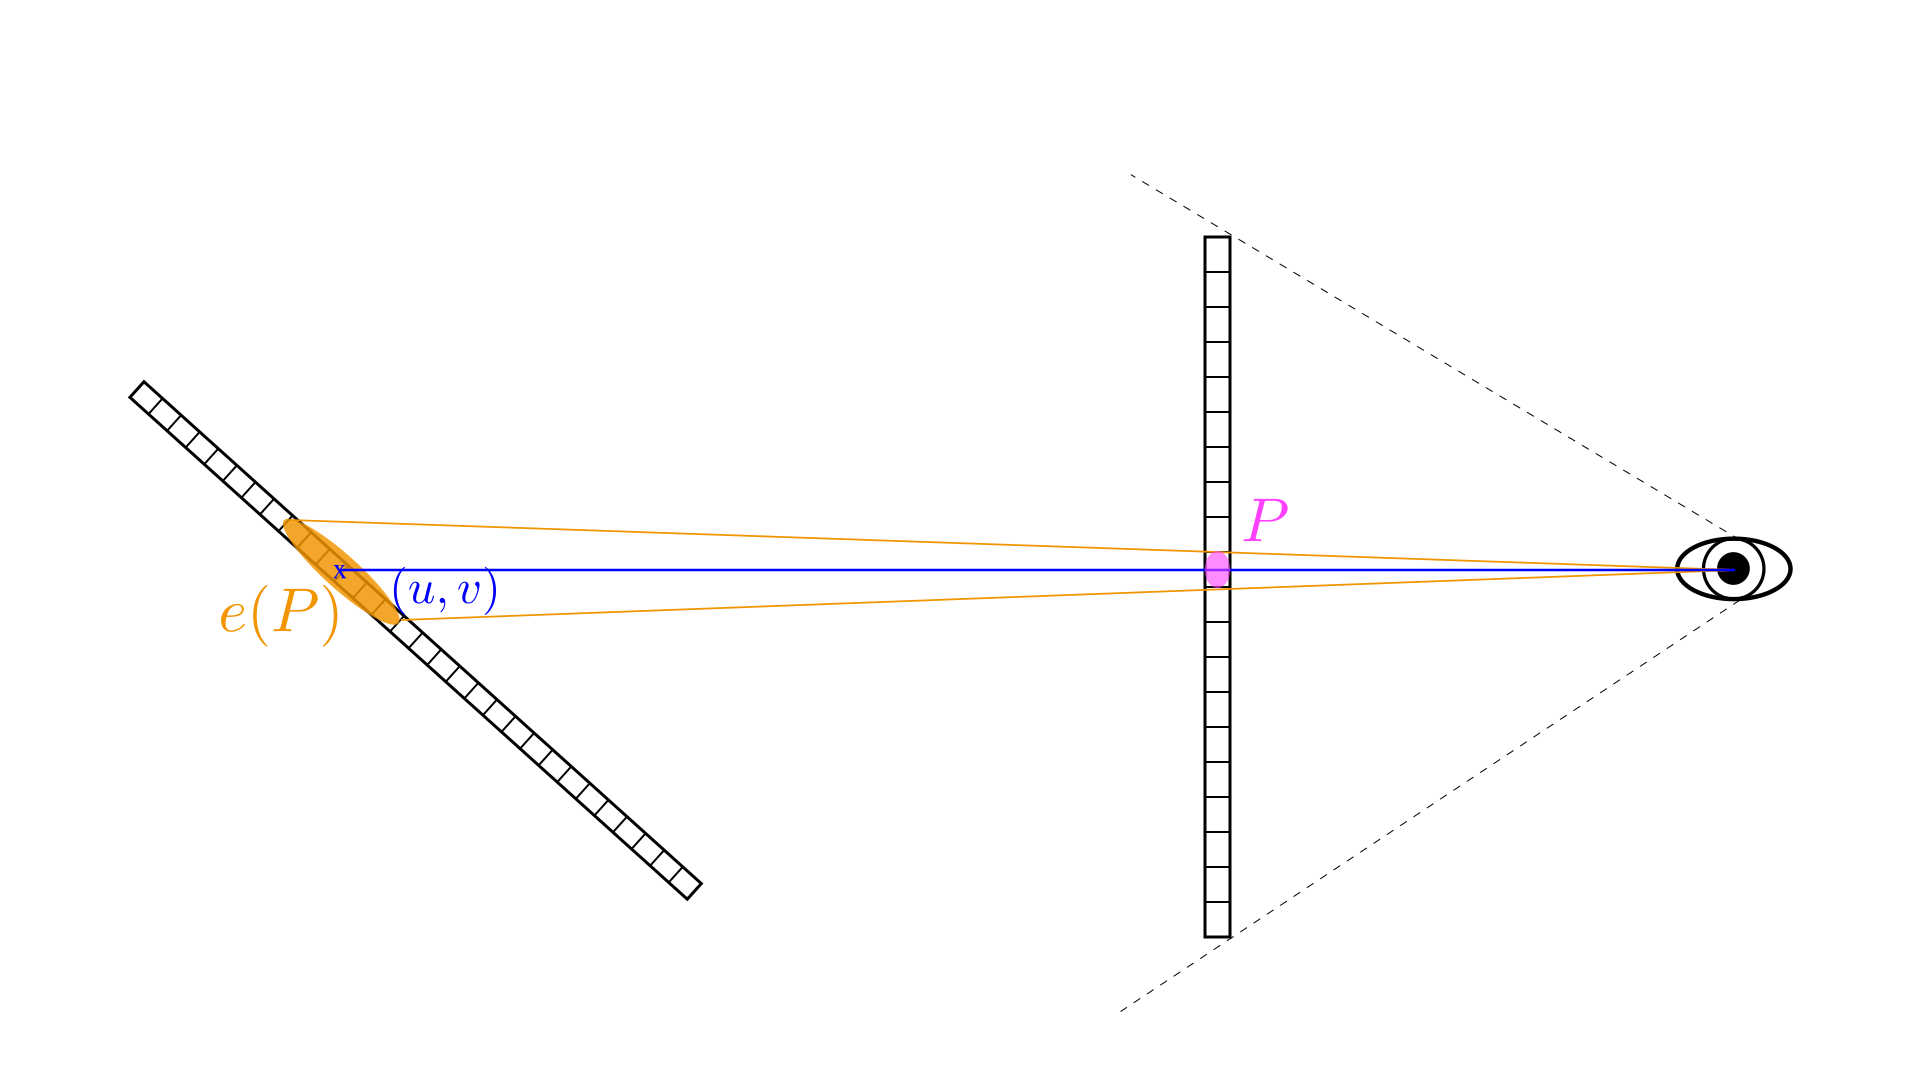
\includegraphics[width=\textwidth]{contenu/resources/images/schema_filtrage}
    \caption[Visualisation du problème d'échantillonnage lors du rendu par rastérisation]{À cette distance de l'écran, l'empreinte du fragment $e(P)$ couvre plusieurs texels. Les coordonnées $(u, v)$ ne sont pas suffisantes pour capturer toute l'information.}
    \label{fig:aliasing}
\end{figure}

Il faut alors employer des méthodes dites de filtrage pour corriger l'échantillonnage, car la différence de taille entre les fragments et les texels cause des artefacts visuels appelés repliement de spectre (\textit{aliasing} en Anglais). Pour des textures standards, il existe différentes méthodes de filtrages utilisées couramment.

\begin{itemize}
    \item \textbf{Sur-échantillonnage} : lorsque le fragment est plus petit que le texel, plusieurs fragments voisins ont la même valeur. Cela donne un aspect crénelé, avec les contours des objet en escalier. La solution idéale dans ce cas serait d'augmenter la résolution de la texture utilisée ; ce n'est cependant pas tout le temps possible. Comme alternative, au lieu d'attribuer au fragment la valeur du texel correspondant, on interpole la valeur des quatre texels voisins. On réduit l'aspect pixélisé, au prix d'un échantillonnage plus coûteux et d'un effet de flou sur l'image. 
    \item \textbf{Sous-échantillonnage} : lorsqu'un fragment est plus grand qu'un texel~\ref{fig:aliasing}, et qu'il en recouvre plusieurs, alors plusieurs fragments voisins peuvent être très espacés sur la texture, et on perd l'information des texels entre. De loin, on aperçoit un motif de moiré et l'image scintille lorsque l'on change légèrement l'angle de vue. La solution idéale serait alors de prendre en compte tous les texels touchés, et faire une intégrale de la valeur de la texture sur toute la surface couverte par le fragment, ce qui est très souvent irréalisable. L'alternative classique consiste à pré-calculer différentes échelles de la texture utilisée, appelées MIP maps, et de trouver l'échelle adéquate de telle sorte qu'un texel ait la même taille qu'un fragment. L'échantillonnage est plus lourd et on prend plus d'espace mémoire pour stocker les MIP maps, mais la texture est mieux rendue de loin.
\end{itemize}


\begin{figure}
    \centering
    \begin{subfigure}[b]{.45\textwidth}
        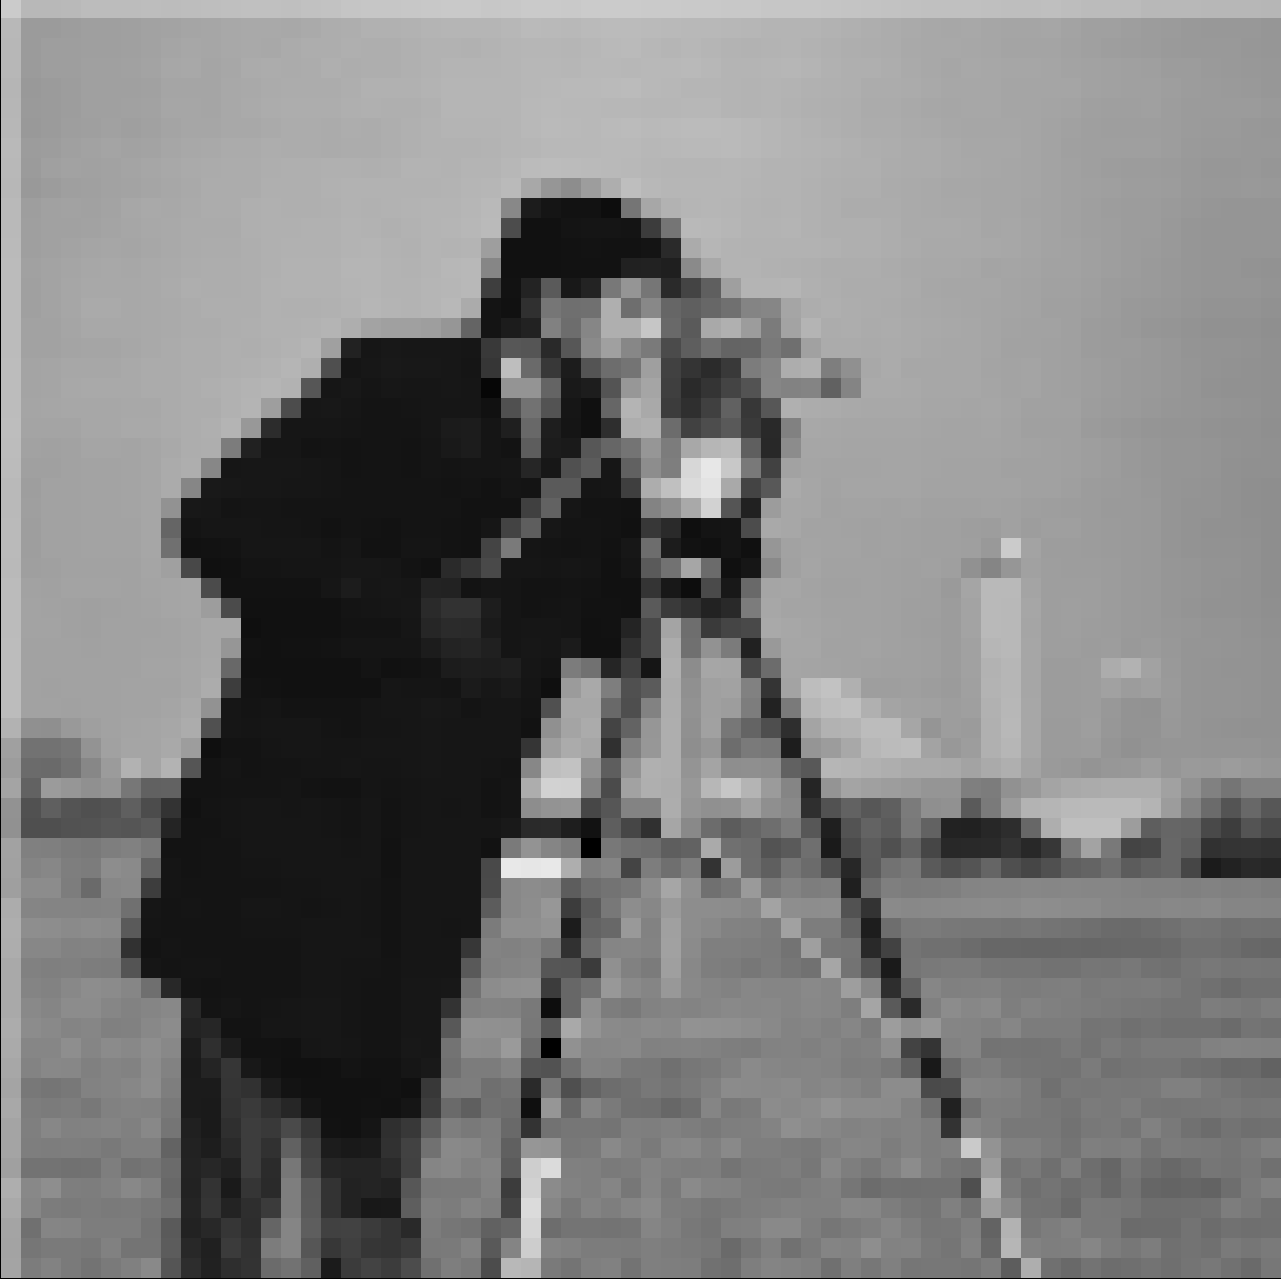
\includegraphics[width=\textwidth]{contenu/resources/images/cameraman_nearest}
        \caption{Sans filtrage}
    \end{subfigure}
    \hfill
    \begin{subfigure}[b]{.45\textwidth}
        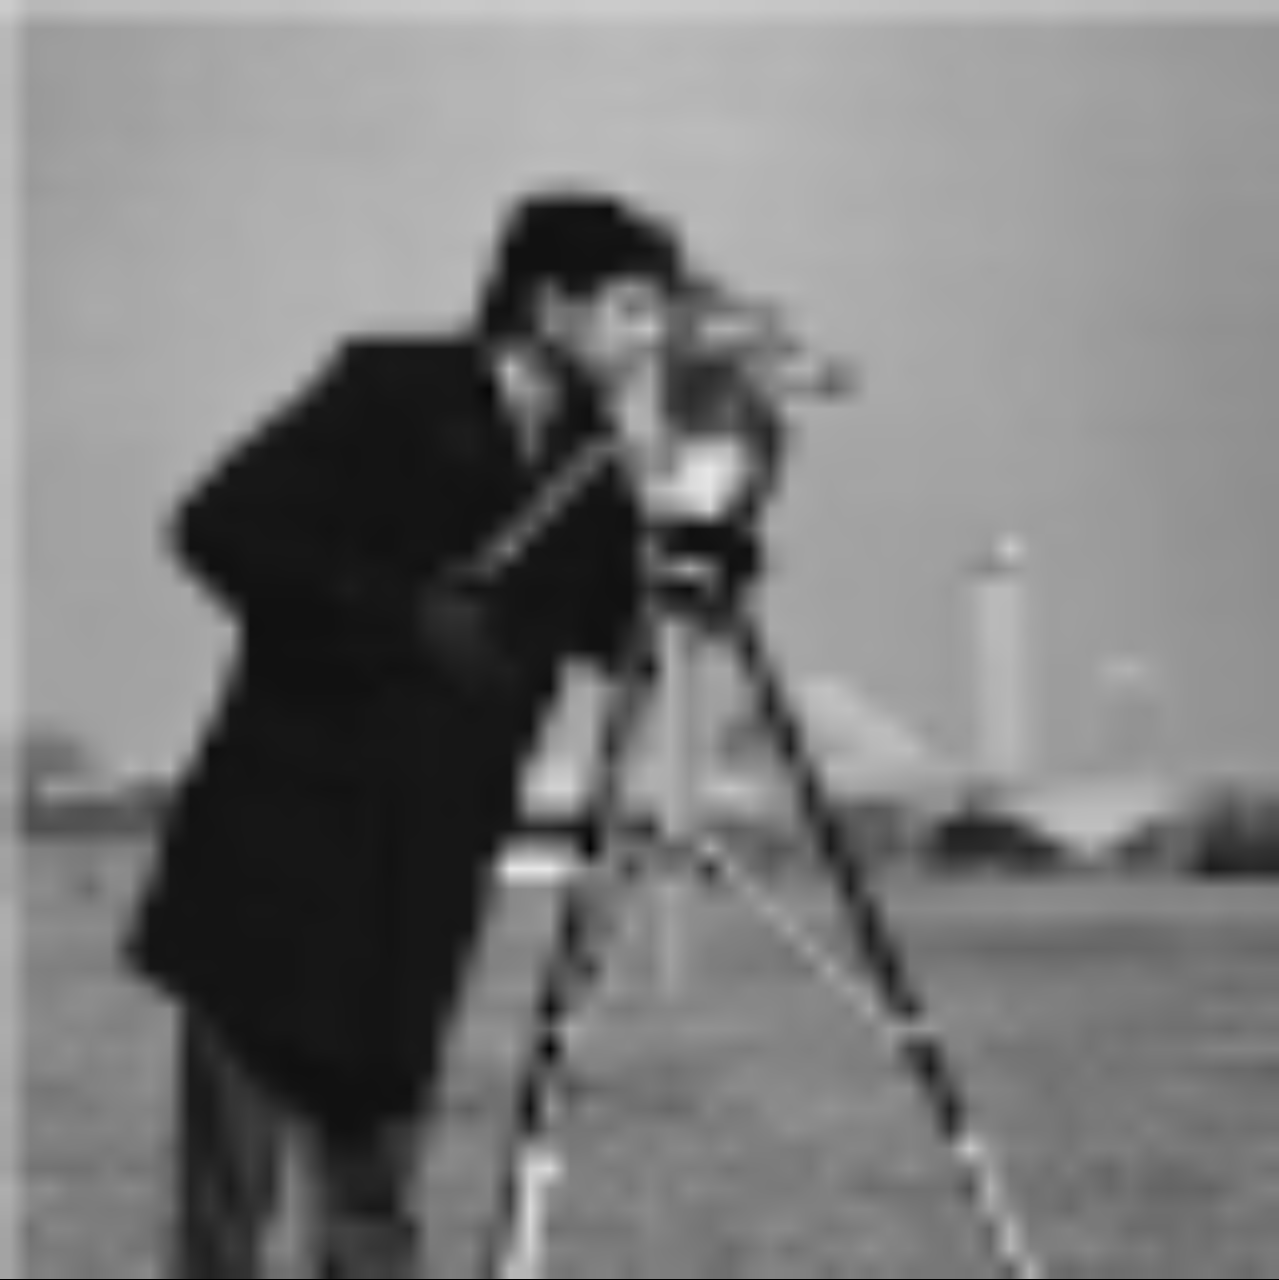
\includegraphics[width=\textwidth]{contenu/resources/images/cameraman_linear}
         \caption{Avec filtrage linéaire}
     \end{subfigure}
    \caption{Filtrer correctement est un enjeu majeur dans l'utilisation des textures}
    \label{fig:filtrage}
\end{figure}

{\color{red}Pertinence de ce paragraphe ?}
De nombreuses méthodes de filtrage plus élaborées sont employées pour obtenir des résultats de meilleur qualité, ou pour filtrer des textures plus compliquées. Par exemple quand les textures ne sont plus des images pré-déterminées à l'avance, mais qu'elles sont générées au moment du rendu.

\section{Synthèse de texture}

Bien souvent, les surfaces que l'on souhaite couvrir sont de grande taille, par exemple des sols. Produire et stocker des textures de même taille que les surfaces n'est pas toujours envisageable, le coût en temps de création et en empreinte mémoire est trop élevé. Étirer les textures en utilisant les coordonnées UV est une solution, qui atteint cependant ses limites assez rapidement : on remarque très facilement qu'une texture de plus basse résolution est utilisée. En rendu intéractif, on résoud le problème en synthétisant directement une texture de taille adaptée à notre surface. On peut catégoriser les types de texture existants de plusieurs manières ; pour le présent manuscrit, nous les distinguerons selon le niveau d'organisation des éléments qui les compose~\ref{fig:échelle-structure}.

\subsection*{Algorithme de synthèse}

On appelle synthèse de texture un procédé qui permet de produire une texture de taille arbitraire, pouvant prendre en argument des paramètres de différente nature. Par extension, on qualifie aussi de synthèse le résultat d'un algorithme de synthèse. Les avantages à utiliser un procédé de synthèse sont multiples. La texture générée est infinie, il est donc facile de l'appliquer à des surfaces de taille quelconque, avec la résolution désirée. De plus, il n'est pas nécessaire de stocker la texture d'avance en mémoire puisqu'on l'évalue au vol, on réduit donc l'empreinte mémoire.

% Enfin, on a un grand degré de contrôle sur l'apparence de nos objets, même au sein d'une scène intéractive.

\begin{figure}[H]
    \centering
    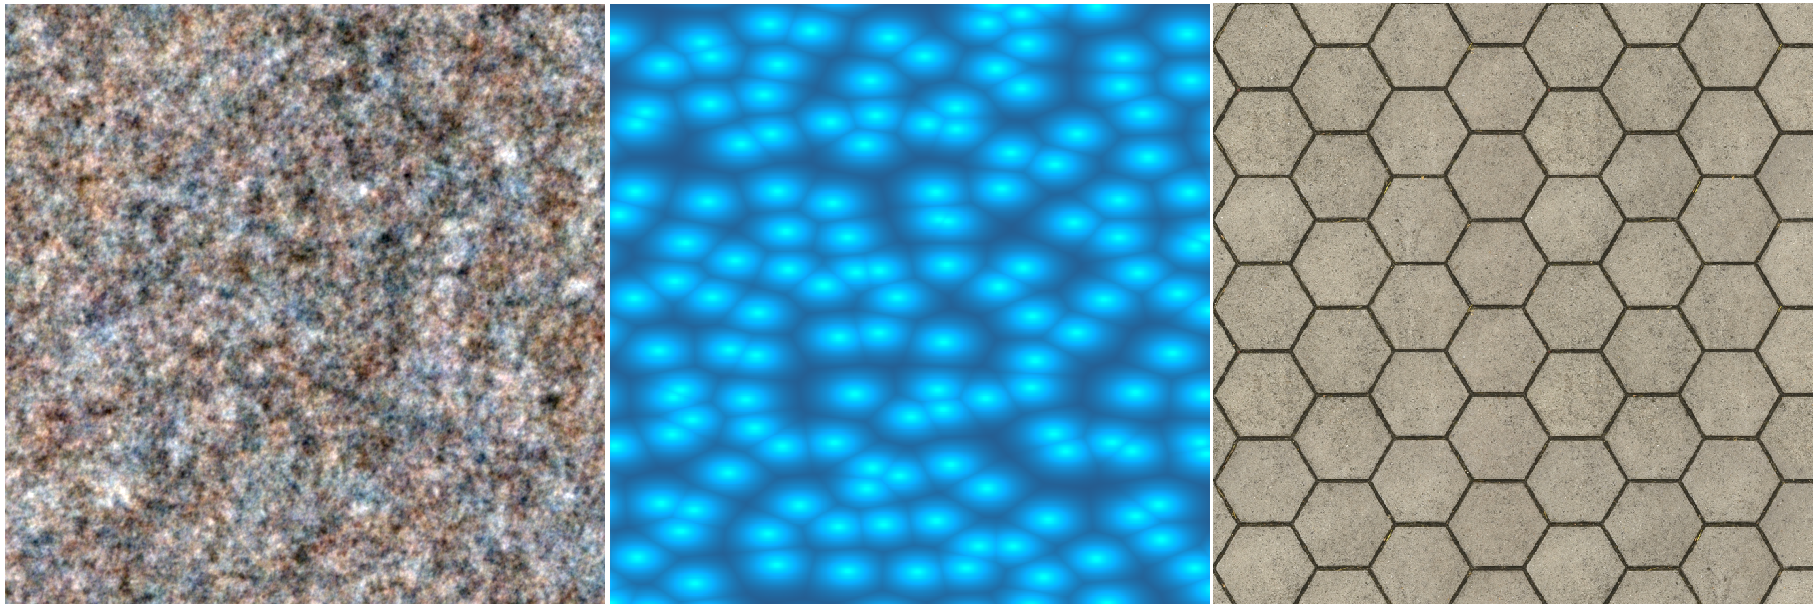
\includegraphics[width=\textwidth]{contenu/resources/images/structure_scale}
    \caption[Classification des textures selon leur niveau de structure]{Les textures peuvent être classées selon leur niveau de structure : stochastiques ou gaussiennes (gauche), semi-régulières (milieu), ou structurées (droite)}
    \label{fig:échelle-structure}
\end{figure}

Il existe plusieurs types de synthèses différentes, qui produisent des types de textures différentes. Une première distinction majeure que l'on peut faire est, comme pour le rendu, entre une synthèse hors-ligne et une synthèse en temps réel. Les ressources en temps et en puissance de calcul impliquées diffèrent, les enjeux ne sont donc souvent pas les mêmes. Nos travaux se focalisent sur le rendu et la synthèse temps-réel, on écarte donc de ce manuscrit les synthèses hors-ligne, comme par exemple les synthèses par optimisation ou par apprentissage profond (ou tout autre forme de réseau de neurones). Les algorithmes auxquels on s'intéresse ont comme contraintes de pouvoir s'exécuter pendant le rendu, sans que le budget de temps du rendu dépasse le seuil établi. Pour rentrer dans ces contraintes de temps, on exploite la puissance des GPUs, et notamment leur aspect hautement parallélisable. Les algorithmes de synthèse doivent donc pouvoir s'exécuter de manière parallèle, chaque texel doit pouvoir se calculer indépendamment des texels voisins ou à l'aide du voisinage proche uniquement.
{\color{red}PARLER DE la métrique des accès texture pour avoir une estimation de la vitesse ?}


\subsection*{Synthèse temps-réel} % / Types de synthèse

Sous ces contraintes d'efficacité et de rapidité, de nombreux algorithmes subsistent ; deux grandes catégories sont la synthèse par ré-organisation et la synthèse par convolution.

\subsubsection{Synthèse par réorganisation}

Le but d'une synthèse par ré-organisation est de reproduire un extrait de texture donné en entrée en réutilisant et réagençant des morceaux dits « tuiles », de l'exemple. Plusieurs paramètres commme la taille, découpe, forme, et disposition des tuiles peuvent être modifiés pour faire varier la synthèse. L'exemple le plus simple de synthèse par réorganisation est le pavage périodique : on répète simplement la texture d'entrée, qui doit être périodique, jusqu'à couvrir la surface désirée. Cette méthode, bien que très rapide, est de faible qualité. Des artefacts visuels sont facilement visibles car les motifs sont simplement répétés, il n'y a pas de variation au sein de la texture générée.

{\color{red}TODO include image pavage periodique (warframe ? outer wilds alpha giants deep)}
\begin{figure}
    \centering
    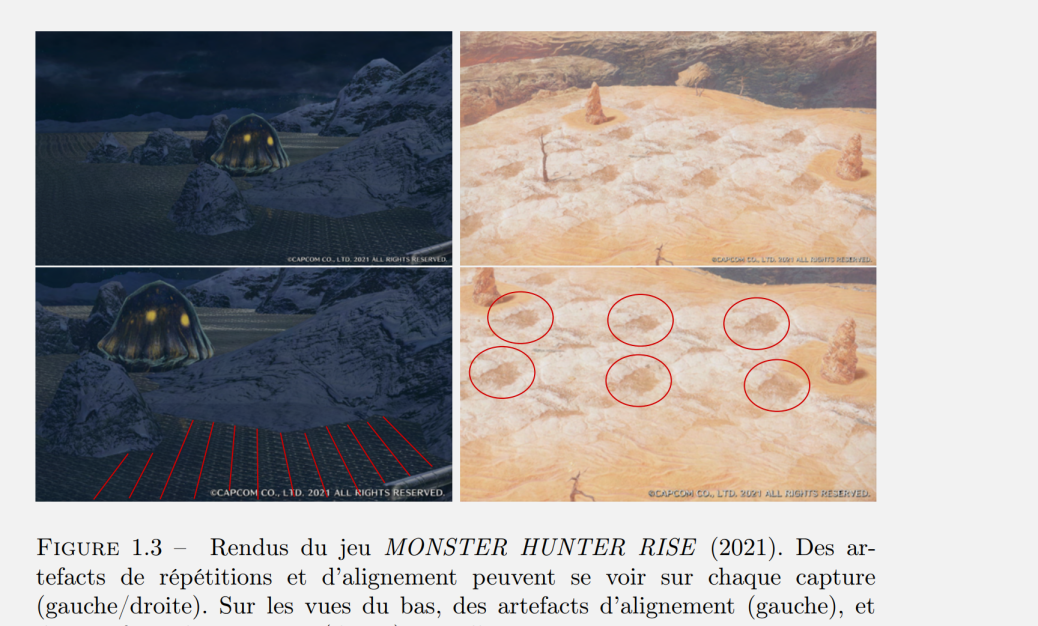
\includegraphics[width=\textwidth]{contenu/resources/images/periodic_tiling}
    \caption[Artefacts d'alignement créés par le pavage périodique]{Artefacts d'alignement créés par le pavage périodique, \textit{Monster Hunter Rise} (2021), Capcom. Crédits à N. Lutz~\cite{lutz_processus_2021} pour l'image}
    \label{fig:pavage_periodique}
\end{figure}

On préfère en général prendre des tuiles plus petites et mieux les mélanger~\cite{heitz_high-performance_2018} afin de d'obtenir de la variété et d'éviter la répétition de motifs saillants. 


\subsubsection{Synthèse par convolution}

L'objectif d'une synthèse par convolution est de construire une texture en disposant des motifs, appelés noyaux, selon une distribution statitique. Le choix du noyau, de la distribution, ainsi que de la méthode de mélange, sont les paramètres à ajuster pour contrôler la synthèse. Une pratique habituelle de la synthèse par convolution est de choisir comme noyau une somme d'ondelettes (typiquement des cosinus) spatialement constraintes et à orientation aléatoire, et de contrôler les fréquences des ondelettes utilisées~\cite{tricard_procedural_2019}. En sélectionnant les fréquences, on a un contrôle sur le contenu fréquentiel présent dans la texture produite, ce qui permet une bonne maîtrise de l'apparence générée~\cite{gilet_local_2014}.

% DIRE QUE LA SYNTHESE DE MOTIFS OU DE STRUCTURE EST ENCORE TRES COMPLIQUEE
Les méthodes existantes de synthèse ne fonctionnent cependant pas bien lorsque la cible contient des motifs organisés ou de la répétition. Quelques tentatives ont été faites~\cite{lutz_cyclostationary-gaussian_2021} pour synthétiser des textures présentant une forme de structure et régularité, mais en dehors de configurations présentant des caractéristiques particulières, comme une certaine périodicité, la synthèse de structure irrégulière est compliquée.

% \section{Génération procédurale} % Non-nécessaire ? De quoi on parle ici sinon ?

% \section{Bruit procédural}

\section{Analyse multi-résolutionnelle locale}

Une des raisons pour lesquelles la synthèse de textures contenant de la structure est difficile est qu'il faut préserver certaines relations entre les texels de l'image pour garder la structure. Savoir quelles relations préserver, pour garder la structure de l'image, et quelles relations supprimer, pour ajouter de la variation dans la synthèse, est très délicat, surtout dans le contexte du temps-réel. L'idée explorée dans cette recherche est d'appliquer des outils de l'analyse d'image, outils capables d'extraire des caractéristiques d'une image par l'analyse de relations intra-image, à des processus de synthèse.

\subsection*{Notion de structure}

La structure d'une image désigne comment les différentes parties de l'image sont agencées les unes par rapport aux autres, comment les éléments de l'image forment certains schémas ou présentent une certaine forme de régularité. Ces relations sont présentes à différents niveaux d'échelle, on a donc différents niveaux de structure. Savoir quels niveaux préserver et comment est important pour reproduire les caractéristiques désirés de la texture.

\begin{figure}[h!]
    \centering
    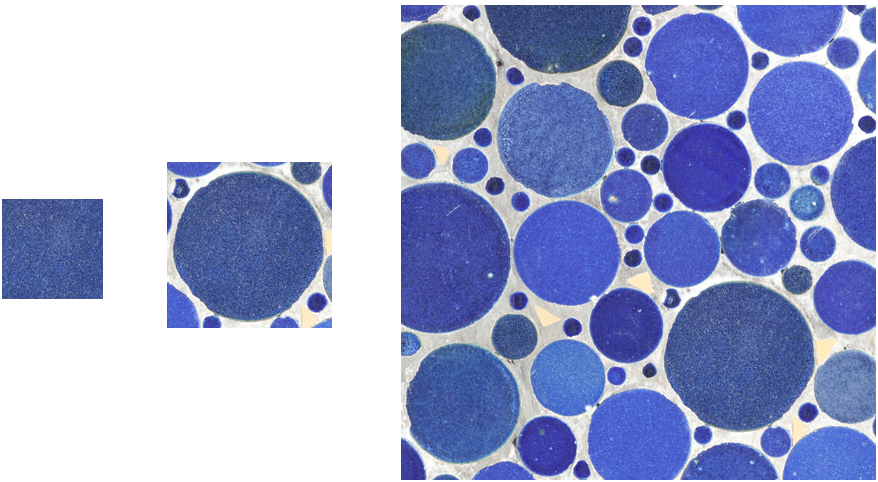
\includegraphics[width=.85\linewidth]{contenu/resources/images/structure_level}
    \caption{Différents niveaux de structure au sein d'une image}
    \label{fig:structure_level}
\end{figure}

\subsection*{Congruence de phases}

Lorsque l'on veut préserver la structure d'une image, les éléments saillants tels que des coins et des lignes, ou plus généralement des bords, sont compliqués à reproduire. On appelle bord une région frontière entre un objet et un autre élément de l'image, comme l'arrière plan ou un autre objet. Visuellement, un bord se distingue facilement par un changement brusque de luminosité. Ces changements sont cependant plus difficiles à détecter automatiquement, car le seuil minimum de contraste entre des pixels voisins n'est pas toujours le même, dépendemment de si le bord est franc ou flou. Une approche intéressante est d'utiliser des informations du domaine fréquentiel pour caractériser des bords.

\bigskip

Lorsqu'une image est décomposée dans le domaine de Fourier, on retrouve de nombreuses informations sur la structure dans la phase~\cite{oppenheim_importance_1981}. En explorant le rôle de la phase, Kovesi a mis au point un outil de détection de d'éléments caractéristiques~\cite{kovesi_image_1995} basé sur le modèle physiologiquement réaliste d'énergie locale de Morrone et al.~\cite{morrone_feature_1987, morrone_feature_1988}. Ce modèle postule que les éléments caractéristiques sont présents dans une image là où les composants de Fourier sont maximalement en phase. La congruence de phase qui dérive du modèle d'énergie locale est une grandeur qui quantifie cet alignement. Elle donne lieu à un outil de détection plus robuste que ceux développés auparavant, qui sont souvent sensibles au niveau d'illumination et de grossissement, et nécessitent donc une connaissance a priori des images étudiées. C'est ce modèle de congruence de phase que nous avons repris et essayé d'adapter à la synthèse de texture.

\begin{figure}[h]
    \centering
    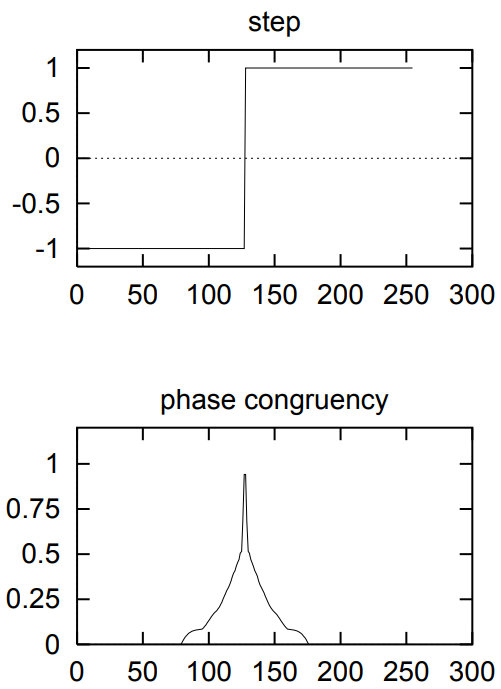
\includegraphics[width=.35\linewidth]{contenu/resources/images/pc_1d_kovesi}
    \caption[Congruence de phase pour un signal 1D]{Congruence de phase pour un signal 1D, Kovesi (1995)~\cite{kovesi_image_1995}}
    \label{fig:pc_1d_kovesi}
\end{figure}

% TODO Transformée de Riesz
Pour détecter un alignement de phase, il est nécessaire d'avoir un modèle donnant des informations locales sur notre image. Kovesi utilise pour cela une banque de filtres à orientation variable. Nous utilisons à la place le modèle mathématique de la transformée de Riesz, qui permet de décomposer une image dans un espace différent, similairement à la transformée de Fourier mais avec des informations locales, au niveau du texel (on rappelle que la transformation de Fourier fournit des informations fréquentiellement locales, mais spatialement globales). Utiliser cette transformée nous permet ainsi d'étudier la présence et préservation de relations dans un autre espace que le domaine spatial, et donc de mieux comprendre et caractériser nos images.

\subsection*{Analyse multi-échelle}

Un objectif de notre méthode est de pouvoir agir avec précision sur certains niveaux d'échelle de structure ciblés. On effectue pour cela une analyse multi-résolutionnelle, qui permet de distinguer des caractéristiques de différentes taille de notre image. On décompose notre image en pyramide d'images, ce qui nous permet d'étudier les différences de détails entre les différents niveaux d'échelle.

\section{Plan} % / problématique

Ce manuscrit est organisé comme suit :

\begin{itemize}
%    \item revue de l'état de l'art de la synthèse de texture temps réel,
    \item explication de la théorie de Riesz et du modèle d'analyse multi-échelle local qui en découle,
    \item application à l'échange de contenu variable.
\end{itemize}